\documentclass{article}
\usepackage[utf8]{inputenc}
\usepackage{amsmath}
\usepackage{amsfonts}
\usepackage{graphicx}
\usepackage[letterpaper, total={7.5in, 9in}]{geometry}

\title{Stochastic Processes}
\author{Grant Smith }
\date{Spring 2022}

\begin{document}

\maketitle

\section{Primer on Random Variables and Conditional Random Variables}

In this section, I want to explain how if two random variables ($X_1$ and $X_2$) are defined on the same event space, observing one random variable, say $X_1$, filters your event space into a smaller event space, and now there is a new random variable that is $X_2$ restricted to that smaller event space. Let's call the value we observe $x_1$.Also note that the probability measure defined on the original event space is now modified to a new measure which depends on the observed value of $X_1$.  This measure (of course) adds up to 1, and those elements in the event space previously added up to less than or equal to 1, so in general they get bigger, but the probability of each element does not necessarily increase.  Also, they are not scaled linearly or anything like that -- we do not know how they change until we know the two random variables.  The new, restricted, event space is $X_1^{-1}(x_1)$, which means it is the inverse image of $x_1$ under the random variable (aka function) $X_1$.  Our notation for this is $X_2 | X_1 = x_1$.  


\section{Stochastic Process Introduction}

I want to develop a little intuition between how we think about stochastic processes, for example, the stock market, and how they're defined in a probability book.  First of all, here is a picture:

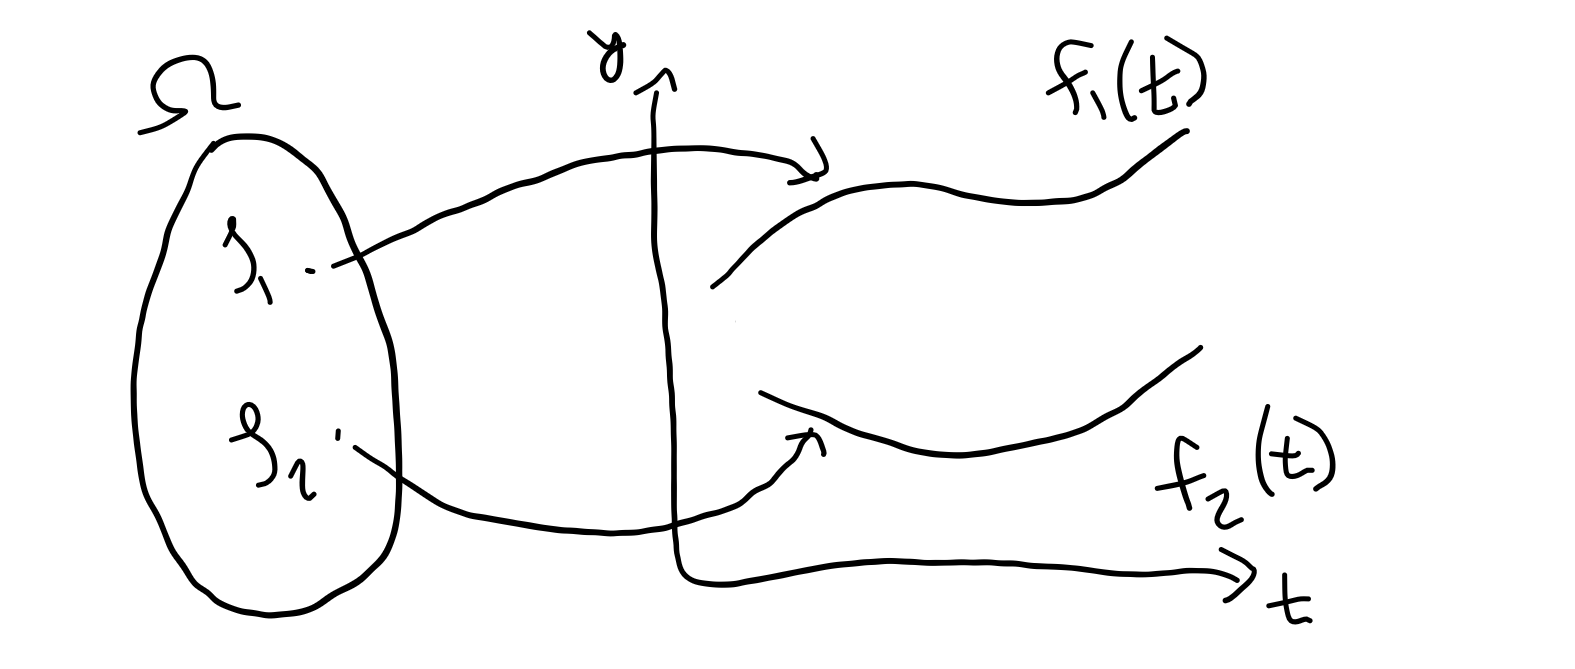
\includegraphics[width=4in]{stochastic_ image.png}
\centering

We have a sample space, $\Omega$, and from that sample space, we map to functions of time (or anything else you want).  We call it a stochastic process, but all it is is a function from a sample space to a space of functions.  The notation is $X_t$, but what's under the hood is the following:

$$X_t = x : \Omega \rightarrow \left(\mathbb{R}^+ \rightarrow  \mathbb{R} \right)$$ 

But we don't really perceive that sample space.  What we perceive (for example when observing the stock market) is that we've observed a process up to a certain time, and we don't know what's going to happen next.  How does that fit into the framework above? Let's start with a picture of a stochastic process.  Here it is, and ignore the 3.5 for now. We'll use it in about two paragraphs.

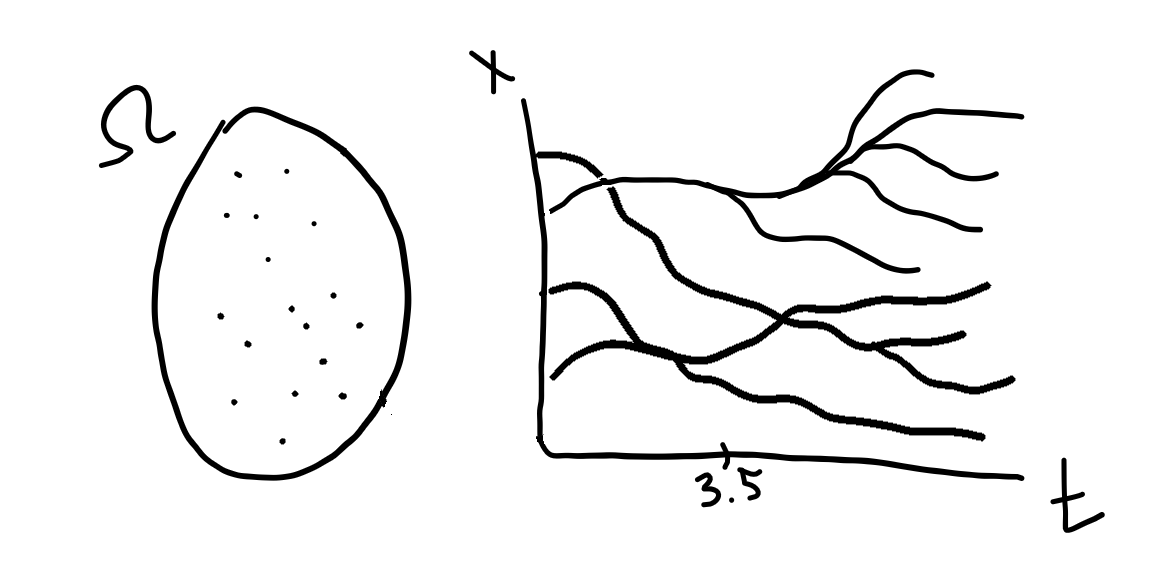
\includegraphics[width=4in]{filtration_part_1.png}
\centering

Let's say this is a stock price over time, and we'll call it $X_t$.  The picture on the right is all the possible trajectories, and the sample space on the left has a corresponding event for each trajectory (I didn't count, so the dots and the trajectories probably don't align, but that's okay).

At our initial time, we have no idea which of these trajectories the stock will take.  But then let's wait a little bit (wait until time 3.5) and observe the price.  Let's say the trajectory we observe is the following:

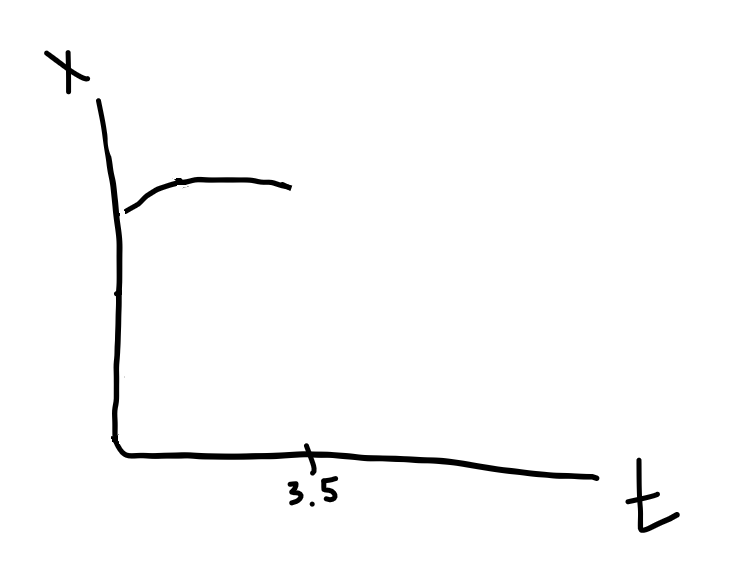
\includegraphics[width=2.2in]{filtration_part_2.png}
\centering

So now we have information about which of the original trajectories are still possible, and which ones are impossible. This is called a filtration, and in our case, we have the filtration at time 3.5, so we will call it$\mathcal{F}_{3.5}$, but in general, it would be $\mathcal{F}_{t}$.

So now we want to figure out what happens to our stochastic process $X_t$ given the information (aka filtration) we know at time 3.5. What the filtration does is filter out all the trajectories that cannot be the case, and it leaves in all the remaining possible trajectories.  The picture is:

\includegraphics[width=4in]{filtration_part_3.png}
\centering

You'll notice that the trajectories that don't align with our filtration are gray, and the events in the sample space that correspond to those trajectories are also gray.  And the trajectories that are possible are still black, and their corresponding events are also still black.

This should feel like a conditional probability, and that's exactly what's happening. We want $Y_t := X_t | \mathcal{F}_{3.5}$.  Thus, $Y_t$ is given by the following drawing:

\includegraphics[width=4in]{filtration_part_4.png}
\centering

At this point, we've really explained a lot.  One last part you might be wondering is what would happen if we changed the 3.5.  And you'd be right. So our $Y_t$ is dependent upon our observation duration. So I'll ammend our notation to be $X_t(s) := X_t | \mathcal{F}_{s}$, which means that the stochastic process we get (a.k.a. remaining trajectories) depends on how long we observe.  So we could say that $Y_t = X_t(3.5)$.  So let's draw another picture for another time, say 4.5. We will start with what we've observed by time = 4.5:

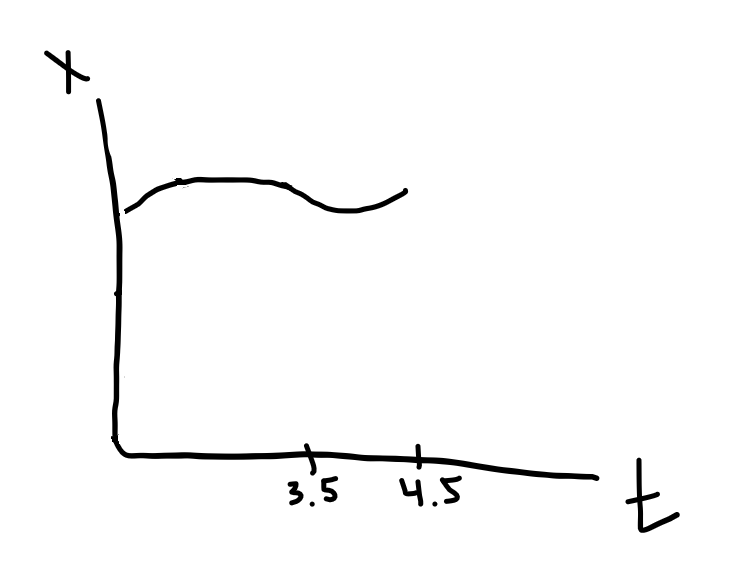
\includegraphics[width=2.2in]{filtration_4.5.png}
\centering

And now we can gray out from the picture of $X_t(3.5)$:

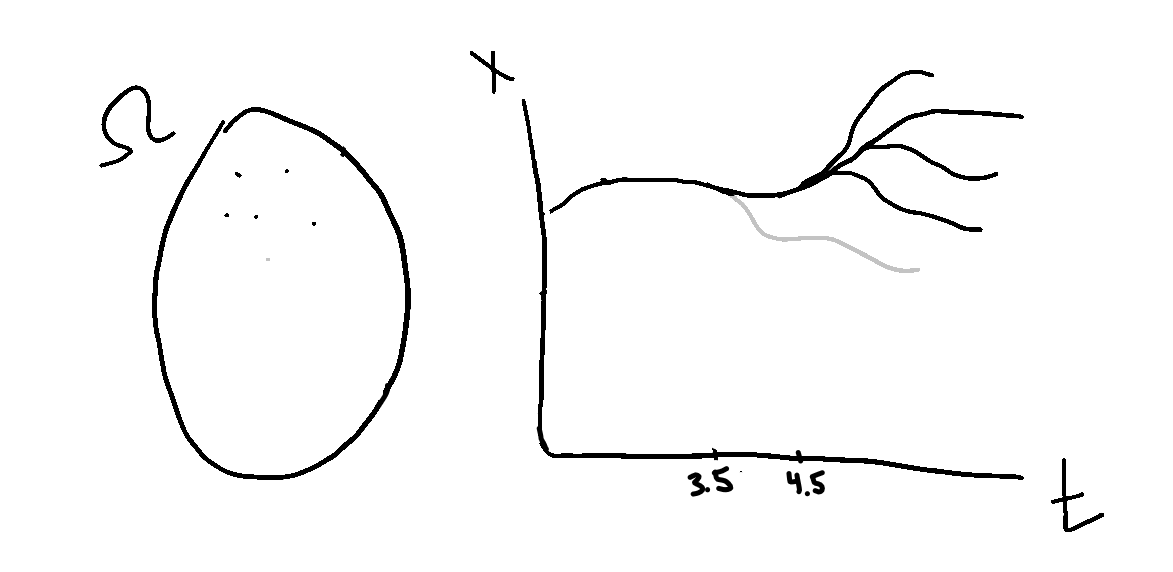
\includegraphics[width=3.2in]{Filtration_grayed_4.5.png}
\centering

And it is hard to see, but one of the elements in the sample space is also grayed out. Which leaves us with our final image of $X_t(4.5)$:

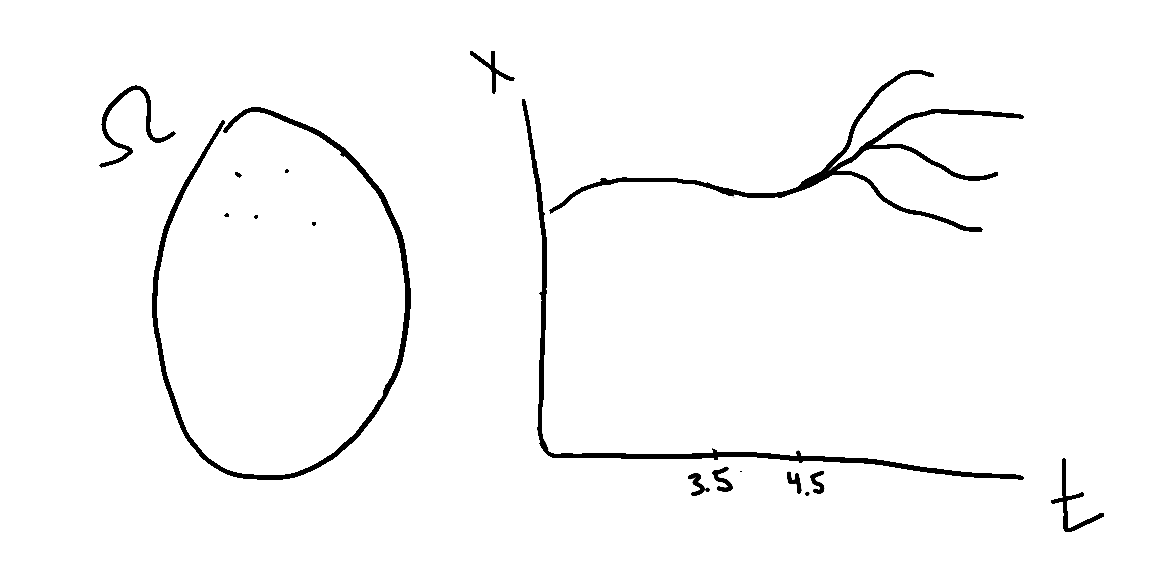
\includegraphics[width=3.2in]{final_4.5.png}
\centering

And this time, it's very clear that I miscounted, and there should only be four elements in the sample space corresponding to the four possible trajectories.

Grant, a note to you, you wanted to write about what $X_t(s)$ looks like???

Lastly, I'm working on making a GeoGebra activity to illustrate this. When it's up, I'll update the link, but here is my account for now: https://www.geogebra.org/u/gsmithapples.

\section{Differentiation and Integration}
Here is the best way I know to think about stochastic differentiation and integration. We'll redraw our picture, and its equation and notation are given below.

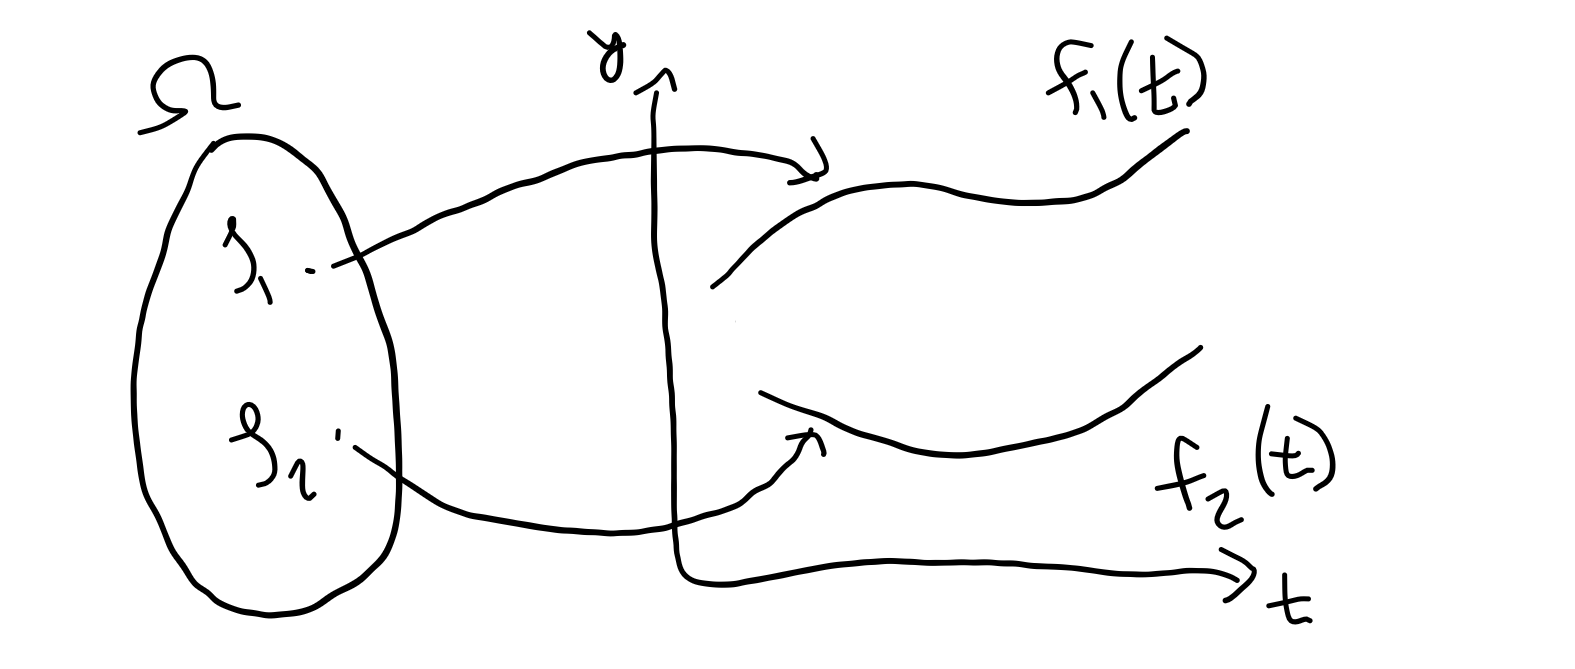
\includegraphics[width=4in]{stochastic_ image.png}
\centering

$$X_t = x : \Omega \rightarrow \left(\mathbb{R}^+ \rightarrow  \mathbb{R} \right)$$ 
$$x(\varsigma_1) = f_1(t)$$
$$x(\varsigma_2) = f_2(t)$$
$$x(\varsigma) = f_\varsigma(t)$$

And note that $x$ is simply a deterministic function.  Also note that we can partially apply and curry however we want, so we also have the following, which will be useful in the following section:

$$X_t = x : \Omega \rightarrow \left(\mathbb{R}^+ \rightarrow  \mathbb{R} \right) = \Omega \rightarrow \mathbb{R}^+ \rightarrow  \mathbb{R} = x :  \left(\Omega  , \mathbb{R}^+\right)\rightarrow  \mathbb{R}$$ 

\subsection{Differentiation}
We have that:

$$X_t' = \frac{\partial}{\partial t}x(\varsigma,t)= \frac{x\left(\varsigma, t + h\right) - x\left(\varsigma, t\right)}{h} = \frac{f_\varsigma\left(t + h\right) - f_\varsigma\left(t\right)}{h} = \frac{df_\varsigma}{dt} =g\left(\varsigma, t\right)$$

Which means that $X_t'$ is just the probability weighted derivatives of the trajectories. Which, just like $x$, is just a deterministiic function of $\varsigma$ and $t$

Side note that this does not work in Brownian Motion because the individual trajectories in Brownian Motion are not differentiable (anywhere).  I think we might be able to do it with some form of a weak derivative, though, just not the regular one.

Also note that we are using the prime notation for a derivative, but it is a partial derivative. That's okay because $\Omega$ isn't necessarily a continuous variable like $t$ is, so when we're differentiating, it is understood that we're differentiating with respect to the only reasonable option, $t$.

\subsection{Integration}
We have that:
$$\int X_t= \int_{s = 0}^{s = t} X_s ds = \int_{s = 0}^{s = t} x\left(\varsigma,s\right) ds = \int_{s = 0}^{s = t} f_\varsigma\left(s\right) ds  = h\left(\varsigma,t\right)$$

Which means that $\int X_t$ is just the probability weighted integrals of the trajectories.  Which, just like $x$ and $g$, is just a deterministic function of $\varsigma$ and $t$

I think we can do this with Brownian Motion because even though Brownian Motion trajectories are not (in the normal sense) differentiable, they are integrable.

\subsection{Differentiation and Integration Example}
Suppose there are only two states of the world, Heads and Tails.  And if Heads is flipped, our world is $x^2 + 2$ and if Tails is flipped, we get $1$.  Our process is:

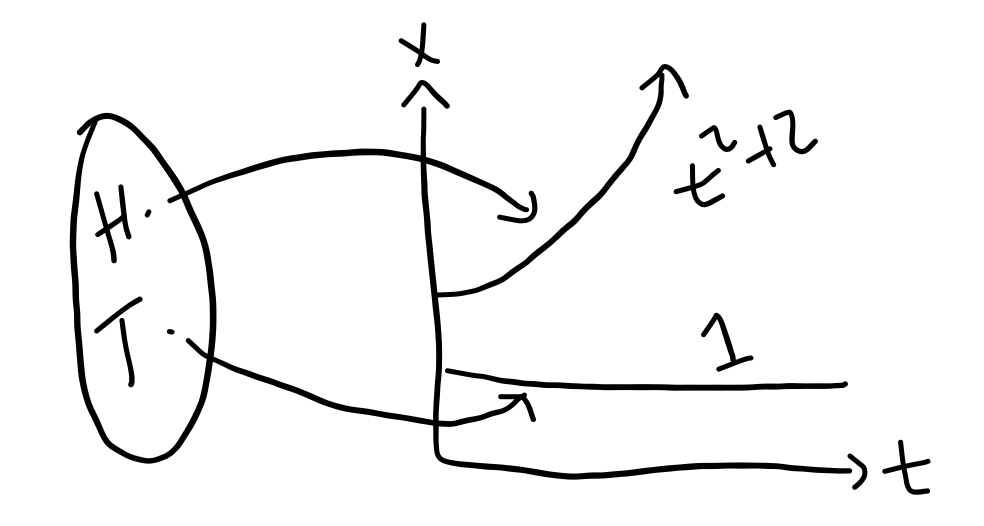
\includegraphics[width=3in]{ExampleProcess.png}
\centering

\[X_t = \begin{cases} 
    t^2 + 2 & H \\
    1 & T 
 \end{cases}
\]

Then we also know:

\[\int X_t = \begin{cases} 
    \frac{1}{3}t^3 + 2t + C_1 & H \\
    t + C_2 & T 
 \end{cases}
\]
\[X_t = \begin{cases} 
    t^2 + 2 & H \\
    1 & T 
 \end{cases}
\]
\[X'_t = \begin{cases} 
    2t & H \\
    0 & T 
 \end{cases}
\]

And those integration constants are deterministic (i.e. they are just numbers).

\section{Ito Processes}

Let's say we have a function $f(t,x)$.  The first argument will stay as time, but the second argument will have a stochastic process $X_t$ plugged in, and the output will now be a stochastic process: $Z_t = f(t,X_t)$.  Our goal will be to find the derivative (or differential) of this process, $dZ_t$. The first thing we will do is expand $f$ using the first two terms of a Taylor Series. That gives us:

$$df = \frac{\partial f}{\partial x} dx + \frac{\partial f}{\partial t} dt + \frac{1}{2}\frac{\partial^2 f}{\partial x^2} dx^2 + \frac{1}{2}\frac{\partial^2 f}{\partial t^2} dt^2 + \frac{\partial^2 f}{\partial x \partial t} dx dt$$

And I think it's helpful to explicitly write the arguments:

$$df(t,x) = \frac{\partial f}{\partial x}(t,x) dx + \frac{\partial f}{\partial t}(t,x) dt + \frac{1}{2}\frac{\partial^2 f}{\partial x^2}(t,x) dx^2 + \frac{1}{2}\frac{\partial^2 f}{\partial t^2}(t,x) dt^2 + \frac{\partial^2 f}{\partial x \partial t}(t,x) dx dt$$

\subsection{Interlude on Taylor Series and Composition}

Let's start as simply as we can: with only one dimension, $f(x)$ and only one degree of approximation:

$$df = \frac{df}{dx} * dx$$

We should probably be a little careful because this is just for intuitive content and it isn't a real statement mathematically.  But continuing, we can explicitly state the dependencies:

$$df(x) = \frac{df}{dx}(x) * dx$$

Notice that $f$ is a function of $x$, but also in this case, we are viewing $df$ as a function, and it is dependent on $x$, so it is $df(x)$ where $df$ is the name of a function.

Now let's make the distance finite. It might be easier to see here because we can make an actual mathematical statement.  The statement is the following (and accompanied with the same thing with explicit dependencies):

$$\Delta f = \frac{df}{dx} * \Delta x$$
$$\Delta f(x, \Delta x) = \frac{df}{dx}(x) * \Delta x$$

Where $\Delta f$ is the name of a function, and it now depends on two things: $x$ and $\Delta x$.  Because we're used to seeing functions and arguments written as single letters, it might be easiest to understand this if we write it as:

$$ f_\Delta = \frac{df}{dx} * h$$
$$ f_\Delta(x, h) = \frac{df}{dx}(x) * h$$



We could also divide both sides by $h$ to get another version of the statement:

$$\frac{ f_\Delta(x, h)}{h} = \frac{df}{dx}(x)$$

Which again, is valid. 

Let's say we wanted to partially evaluate this at, say, 4. We would get

$$ f_\Delta(4, h) = \frac{df}{dx}(4) * h$$

So let's do an example. What if $f(x) = x^2$?  Then $f'(x) = 2x$, and we would have $f_\Delta(x, h) = 2xh$.  We know that if $h = 1$ then we have our standard derivative.




\end{document}
